\chapter{Mesure du temps d'exécution des nombres premiers ayant au plus 12 chiffres}

Le tableau suivant représente le temps d'exécutions des six algorithmes pour des nombres ayant des longueurs différentes (6,7,8,9,10,11,12)
\\
\par
\small
\resizebox{17cm}{!}{
\begin{tabular}{| c | c | c | c | c | c | c | }
    \hline
    Nombre premier &  A1 & A2 & A3 & A4 & A5 & A6   \\
    \hline
 314159    &  0.010000 &	0.001000 & 0.000000 &	0.001000 &	0.000000 &	0.000000
 \\
    \hline
4480649 & 0.066000 &	0.022000 &	0.000000 &	0.020000	& 0.012000 &	0.000000  \\
    \hline
    50943779 & 0.440000	& 0.271000 &	0.000000 &	0.218000 &	0.129000	& 0.000000  \\
    \hline
    999999937 & 8.502600	& 4.378000	& 0.000633	& 7.151200	& 2.185066 &	0.001267 \\
    \hline
    5915587277 & 8.392000 &	5.146000 &	0.001000	& 5.180000	& 2.375000 &	0.000000 \\
    \hline
    41996139943 & 371.614000 &	208.341000 &	0.003000	 & 199.646000 &	100.515000 &	0.003000 \\
    \hline
    100123456789 & 912.519000 &	502.751000 &	0.005000 &	464.866000	& 311.032000	& 0.003000 \\
     \hline
\end{tabular}}
\\
\par
La figure suivante (voir Figure \ref{fig:chart1}) représente les résultats d'executions des six algoritmes pour ces nombres.

\begin{figure}[H]
    \centering
        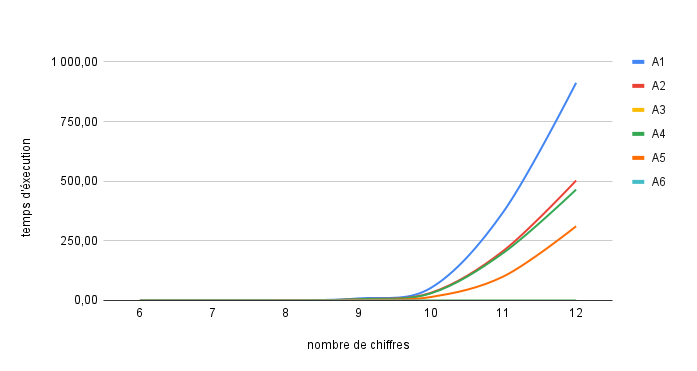
\includegraphics[scale=0.7]{chart1.png}
        \caption{Temps d'exécution des six algorithmes sur 7 nombres de chiffres différents }
    \label{fig:chart1}
\end{figure}
\\ \\
